% Options for packages loaded elsewhere
\PassOptionsToPackage{unicode}{hyperref}
\PassOptionsToPackage{hyphens}{url}
\PassOptionsToPackage{dvipsnames,svgnames,x11names}{xcolor}
%
\documentclass[
  11pt,
]{article}

\usepackage{amsmath,amssymb}
\usepackage{setspace}
\usepackage{iftex}
\ifPDFTeX
  \usepackage[T1]{fontenc}
  \usepackage[utf8]{inputenc}
  \usepackage{textcomp} % provide euro and other symbols
\else % if luatex or xetex
  \usepackage{unicode-math}
  \defaultfontfeatures{Scale=MatchLowercase}
  \defaultfontfeatures[\rmfamily]{Ligatures=TeX,Scale=1}
\fi
\usepackage{lmodern}
\ifPDFTeX\else  
    % xetex/luatex font selection
    \setmainfont[]{Arial}
    \setmonofont[]{DejaVu Sans Mono}
\fi
% Use upquote if available, for straight quotes in verbatim environments
\IfFileExists{upquote.sty}{\usepackage{upquote}}{}
\IfFileExists{microtype.sty}{% use microtype if available
  \usepackage[]{microtype}
  \UseMicrotypeSet[protrusion]{basicmath} % disable protrusion for tt fonts
}{}
\makeatletter
\@ifundefined{KOMAClassName}{% if non-KOMA class
  \IfFileExists{parskip.sty}{%
    \usepackage{parskip}
  }{% else
    \setlength{\parindent}{0pt}
    \setlength{\parskip}{6pt plus 2pt minus 1pt}}
}{% if KOMA class
  \KOMAoptions{parskip=half}}
\makeatother
\usepackage{xcolor}
\usepackage[lmargin=0.8in,rmargin=0.8in,tmargin=0.8in,bmargin=0.8in]{geometry}
\ifLuaTeX
  \usepackage{luacolor}
  \usepackage[soul]{lua-ul}
\else
  \usepackage{soul}
  
\fi
\setlength{\emergencystretch}{3em} % prevent overfull lines
\setcounter{secnumdepth}{-\maxdimen} % remove section numbering
% Make \paragraph and \subparagraph free-standing
\makeatletter
\ifx\paragraph\undefined\else
  \let\oldparagraph\paragraph
  \renewcommand{\paragraph}{
    \@ifstar
      \xxxParagraphStar
      \xxxParagraphNoStar
  }
  \newcommand{\xxxParagraphStar}[1]{\oldparagraph*{#1}\mbox{}}
  \newcommand{\xxxParagraphNoStar}[1]{\oldparagraph{#1}\mbox{}}
\fi
\ifx\subparagraph\undefined\else
  \let\oldsubparagraph\subparagraph
  \renewcommand{\subparagraph}{
    \@ifstar
      \xxxSubParagraphStar
      \xxxSubParagraphNoStar
  }
  \newcommand{\xxxSubParagraphStar}[1]{\oldsubparagraph*{#1}\mbox{}}
  \newcommand{\xxxSubParagraphNoStar}[1]{\oldsubparagraph{#1}\mbox{}}
\fi
\makeatother


\providecommand{\tightlist}{%
  \setlength{\itemsep}{0pt}\setlength{\parskip}{0pt}}\usepackage{longtable,booktabs,array}
\usepackage{calc} % for calculating minipage widths
% Correct order of tables after \paragraph or \subparagraph
\usepackage{etoolbox}
\makeatletter
\patchcmd\longtable{\par}{\if@noskipsec\mbox{}\fi\par}{}{}
\makeatother
% Allow footnotes in longtable head/foot
\IfFileExists{footnotehyper.sty}{\usepackage{footnotehyper}}{\usepackage{footnote}}
\makesavenoteenv{longtable}
\usepackage{graphicx}
\makeatletter
\def\maxwidth{\ifdim\Gin@nat@width>\linewidth\linewidth\else\Gin@nat@width\fi}
\def\maxheight{\ifdim\Gin@nat@height>\textheight\textheight\else\Gin@nat@height\fi}
\makeatother
% Scale images if necessary, so that they will not overflow the page
% margins by default, and it is still possible to overwrite the defaults
% using explicit options in \includegraphics[width, height, ...]{}
\setkeys{Gin}{width=\maxwidth,height=\maxheight,keepaspectratio}
% Set default figure placement to htbp
\makeatletter
\def\fps@figure{htbp}
\makeatother
% definitions for citeproc citations
\NewDocumentCommand\citeproctext{}{}
\NewDocumentCommand\citeproc{mm}{%
  \begingroup\def\citeproctext{#2}\cite{#1}\endgroup}
\makeatletter
 % allow citations to break across lines
 \let\@cite@ofmt\@firstofone
 % avoid brackets around text for \cite:
 \def\@biblabel#1{}
 \def\@cite#1#2{{#1\if@tempswa , #2\fi}}
\makeatother
\newlength{\cslhangindent}
\setlength{\cslhangindent}{1.5em}
\newlength{\csllabelwidth}
\setlength{\csllabelwidth}{3em}
\newenvironment{CSLReferences}[2] % #1 hanging-indent, #2 entry-spacing
 {\begin{list}{}{%
  \setlength{\itemindent}{0pt}
  \setlength{\leftmargin}{0pt}
  \setlength{\parsep}{0pt}
  % turn on hanging indent if param 1 is 1
  \ifodd #1
   \setlength{\leftmargin}{\cslhangindent}
   \setlength{\itemindent}{-1\cslhangindent}
  \fi
  % set entry spacing
  \setlength{\itemsep}{#2\baselineskip}}}
 {\end{list}}
\usepackage{calc}
\newcommand{\CSLBlock}[1]{\hfill\break\parbox[t]{\linewidth}{\strut\ignorespaces#1\strut}}
\newcommand{\CSLLeftMargin}[1]{\parbox[t]{\csllabelwidth}{\strut#1\strut}}
\newcommand{\CSLRightInline}[1]{\parbox[t]{\linewidth - \csllabelwidth}{\strut#1\strut}}
\newcommand{\CSLIndent}[1]{\hspace{\cslhangindent}#1}

\usepackage{lineno}
\makeatletter
\@ifpackageloaded{caption}{}{\usepackage{caption}}
\AtBeginDocument{%
\ifdefined\contentsname
  \renewcommand*\contentsname{Table of contents}
\else
  \newcommand\contentsname{Table of contents}
\fi
\ifdefined\listfigurename
  \renewcommand*\listfigurename{List of Figures}
\else
  \newcommand\listfigurename{List of Figures}
\fi
\ifdefined\listtablename
  \renewcommand*\listtablename{List of Tables}
\else
  \newcommand\listtablename{List of Tables}
\fi
\ifdefined\figurename
  \renewcommand*\figurename{Figure}
\else
  \newcommand\figurename{Figure}
\fi
\ifdefined\tablename
  \renewcommand*\tablename{Table}
\else
  \newcommand\tablename{Table}
\fi
}
\@ifpackageloaded{float}{}{\usepackage{float}}
\floatstyle{ruled}
\@ifundefined{c@chapter}{\newfloat{codelisting}{h}{lop}}{\newfloat{codelisting}{h}{lop}[chapter]}
\floatname{codelisting}{Listing}
\newcommand*\listoflistings{\listof{codelisting}{List of Listings}}
\makeatother
\makeatletter
\makeatother
\makeatletter
\@ifpackageloaded{caption}{}{\usepackage{caption}}
\@ifpackageloaded{subcaption}{}{\usepackage{subcaption}}
\makeatother

\ifLuaTeX
  \usepackage{selnolig}  % disable illegal ligatures
\fi
\usepackage{bookmark}

\IfFileExists{xurl.sty}{\usepackage{xurl}}{} % add URL line breaks if available
\urlstyle{same} % disable monospaced font for URLs
\hypersetup{
  pdftitle={Cell-type diversity and connectome of the ctenophore apical organ},
  colorlinks=true,
  linkcolor={blue},
  filecolor={Maroon},
  citecolor={Blue},
  urlcolor={Blue},
  pdfcreator={LaTeX via pandoc}}


\title{Cell-type diversity and connectome of the ctenophore apical
organ}
\author{}
\date{}

\begin{document}
\maketitle

\linenumbers


\setstretch{1.2}
\hfill\break

Kei Jokura\textsuperscript{1,3,4,*}, Sanja Jasek\textsuperscript{1,2},
Lara Kewalow\textsuperscript{2}, Pawel Burkhardt\textsuperscript{5},
Gáspár Jékely\textsuperscript{1,2,*}\\

\textsuperscript{1}Living Systems Institute, University of Exeter,
Exeter, EX4 4QD, United Kingdom\\
\textsuperscript{2}Heidelberg University, Centre for Organismal Studies
(COS), 69120 Heidelberg, Germany\\
\textsuperscript{3}Exploratory Research Center on Life and Living
Systems (ExCELLS), National Institutes of Natural Sciences, Okazaki,
Japan\\
\textsuperscript{4}National Institute for Basic Biology (NIBB), National
Institutes of Natural Sciences, Okazaki, Japan\\
\textsuperscript{5}Michael Sars Centre, University of Bergen, Norway\\
\textsuperscript{*}Correspondence: jokura@nibb.ac.jp,
gaspar.jekely@cos.uni-heidelberg.de

\subsection{Abstract}\label{abstract}

\textbf{text in bold} \emph{italic} \ul{underline}

\subsection{Introduction}\label{introduction}

First descriptions of AO: (Aronova, 1974)

The lobate ctenophore \emph{Mnemiopsis}

The lithocytes have a large calcium carbonate concretion and\ldots{}
(Tamm, 2014) Living lithocytes are transported along the balancer cilia
to the tip of the statocyst (Noda and Tamm, 2014) The projections of a
group of bridge cells located on two sides of the apical organ forms an
arch and connects the balancers along the tentacular plane (Tamm and
Tamm, 2002).

\subsection{Results}\label{results}

\subsubsection{\texorpdfstring{Volume EM reconstruction of the
\emph{Mnemiopsis} apical
organ}{Volume EM reconstruction of the Mnemiopsis apical organ}}\label{volume-em-reconstruction-of-the-mnemiopsis-apical-organ}

First, we embedded the entire body of the \emph{Mnemiopsis leidyi}
cydippid-stage larvae, five days post-fertilization, in Epon resin
following high-pressure freezing. To reconstruct all synaptic-resolution
connections among the cells comprising the apical organ, also known as
the aboral organ, we prepared approximately 1,000 ultra-thin serial
sections (50 nm thick) from the aboral tip of the larval body embedded
in the resin block. Using a scanning electron microscope (Gemini SEM
500) with a resolution of 2.0 nm/pixel, we imaged only the region
containing the apical organ. Subsequently, 620 of these images were
stitched and aligned using TrakEM2. The resulting volumetric EM dataset
had dimensions of 60 μm × 40 μm × 30 μm. We traced and annotated all
cells in this dataset, ultimately reconstructing 909 cells, each with
both nuclei and cell bodies intact.

Cells containing cilia were traced down to the tips of the cilia, and
basal bodies were annotated accordingly. For neuronal skeletonization,
nodes were placed to interconnect the profiles of the same neuron's
processes across layers, extending the skeleton until all branches were
fully traced. Each node was tagged, and skeletons were named and
assigned multi-level annotations. As described later, many neurons we
identified formed loop-like structures (anastomosed neurons), wherein
separated branches often rejoined either the main trunk or other
branches. In such cases, branch nodes were placed near the closest
existing node and annotated accordingly. The entire skeletonized volume
was composed of 134,591 nodes. However, 88 fragments could not be
attached to somata-associated skeletons. Most of these fragments
represented short skeletal branches that could not be traced beyond gaps
or low-quality layers.

Next, we decided to divide the entire apical organ into four broad
quadrants to facilitate grouping the identified cells. The general body
plan of ctenophores, when viewed from the aboral side, exhibits biradial
symmetry around the positions of the anal pores. This symmetry
corresponds to the four blastomeres present at the four-cell stage
during early embryonic development. We categorized the traced cells into
four quadrants and designated these groups as Q1 through Q4 for clarity
and consistency.

\begin{figure}[H]

{\centering 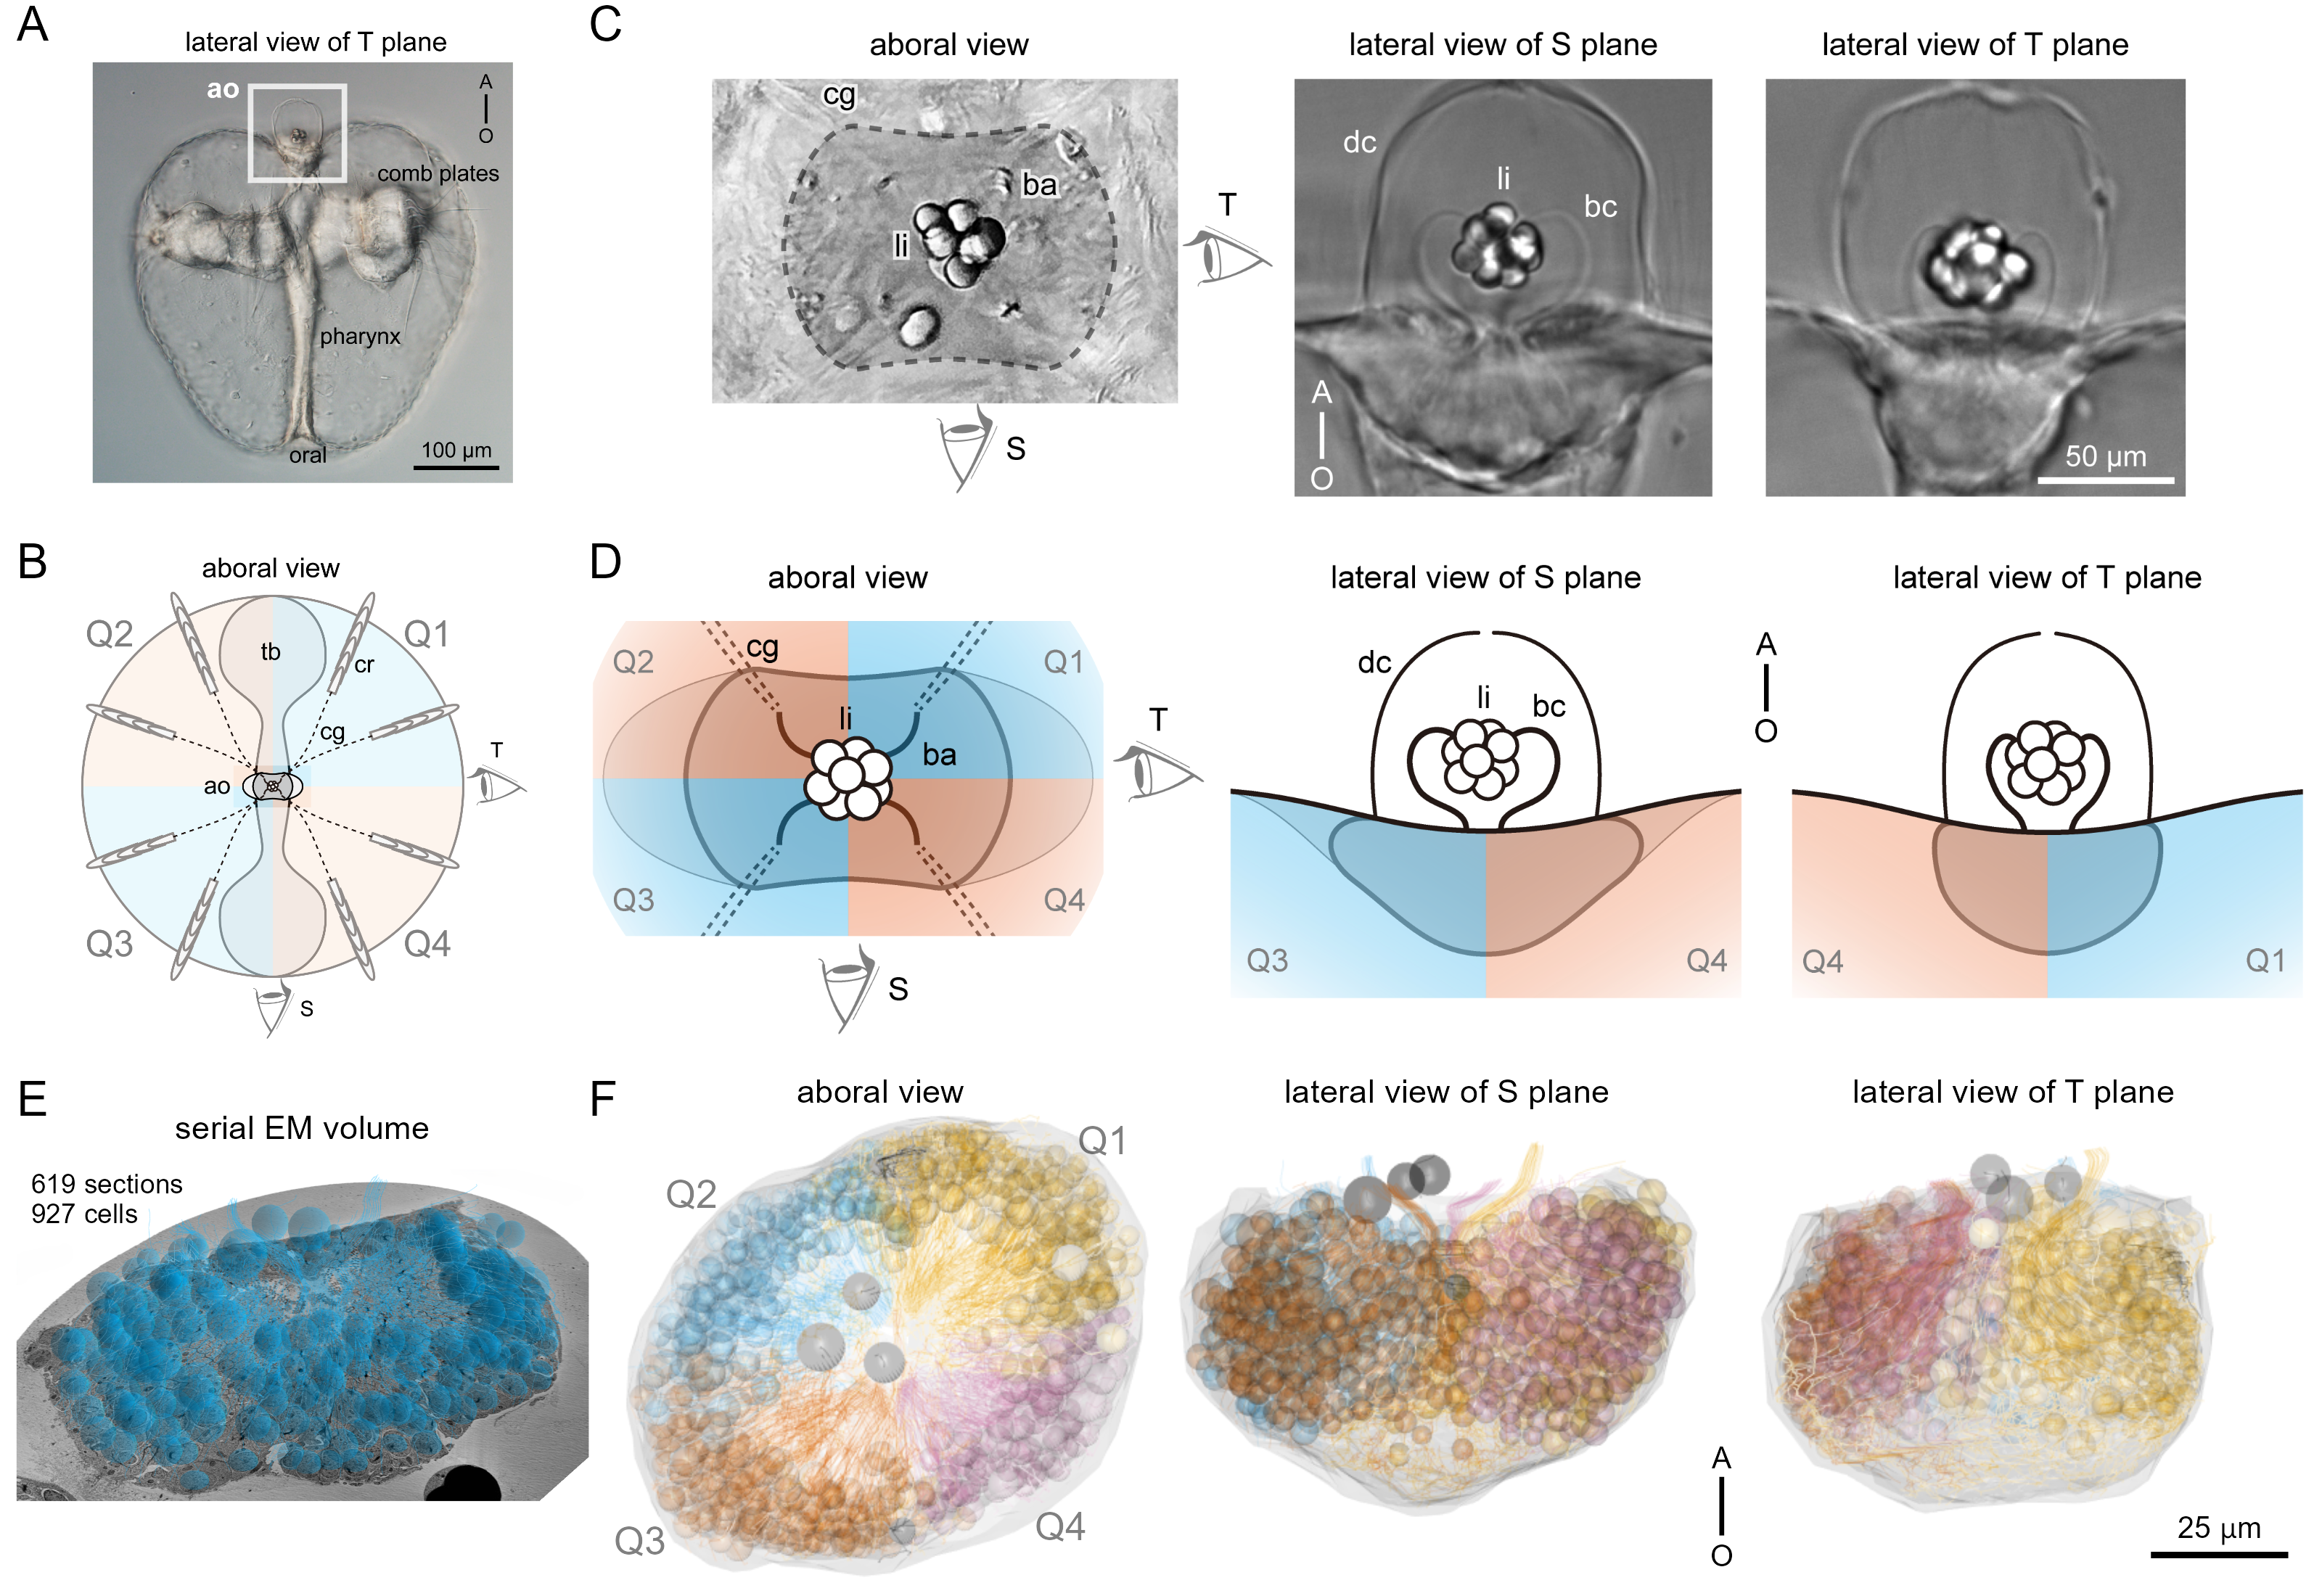
\includegraphics[width=1\textwidth,height=\textheight]{figures/Figure1.png}

}

\caption{\textbf{Figure 1. Title fig 1} pic of a larva, boxed region of
AO, schematic, catmaid pic with slice, dimensions, quadrants, regions,
(A) legend (B) legend.}

\end{figure}%

\subsubsection{Identification of Synaptic Structures in Syncytium
Neurons}\label{identification-of-synaptic-structures-in-syncytium-neurons}

Classical neural staining techniques do not provide clear images of the
neurons at the aboral pole. However, ultrastructural studies have
provided morphological evidence of elements resembling neurons, based on
synaptic structures, located on the epithelial floor of the apical
organs (Hernandez-Nicaise, 1973; Horridge and Mackay, 1964). Based on
these findings, we identified synaptic structures characteristic of
ctenophore neurons in our data, using previously identified pre-synaptic
triad morphological features, such as single-layered vesicles, smooth
endoplasmic reticulum, and tightly packed mitochondria. In our study, we
specifically identified synaptic sites and marked mitochondria (orange)
as synaptic nodes. The regions where synaptic vesicles align were marked
as connectors (light blue arrows) between cells across the membrane.
These connectors link the synaptic nodes of the pre-synaptic
cytoskeleton to the partner nodes of the post-synaptic cytoskeleton. As
previously reported, the specialization of post-synaptic structures in
ctenophores is not apparent, so we recognized synaptic vesicle clusters
on the pre-synaptic membrane as the point of reference. Synapses were
identified as either monoadic or polyadic, with one pre-synaptic neuron
forming connections with one or multiple post-synaptic cells.

As mentioned above, following the identification of the presynaptic
structures, we reconstructed three major Syncytial neurons. Each of
these Syncytial neurons was a cell with multiple nuclei, with membranes
fused by continuous plasma membranes. These neurons are distinct in
morphology from the Syncytial subepithelial nerve net (SNN) neurons with
blebbed morphology previously reconstructed in 3D
(\textbf{Burkhardt\_2023?}). Our findings represent the second
documented discovery of Syncytial neurons in ctenophores. Furthermore,
these neurons exhibited clear morphological differences when compared to
other sensory cells reported in the same study, such as mesogleal
neurons and sensory cells with presynaptic structures and cilia (types
1-4)(\textbf{Burkhardt\_2023?}). Based on their distinct spatial
relationships, we were able to classify these three Syncytial neurons
into two categories. The first type is a larger ``AO neuron\_Q1234,''
which possesses four (or possibly six?) nuclei spanning four quadrants.
It contained X presynaptic structures. The second type consists of ``AO
neuron\_Q12'' and ``AO neuron\_Q34,'' each having two nuclei spanning
two quadrants, and each containing X presynaptic structures.

\begin{figure}[H]

{\centering 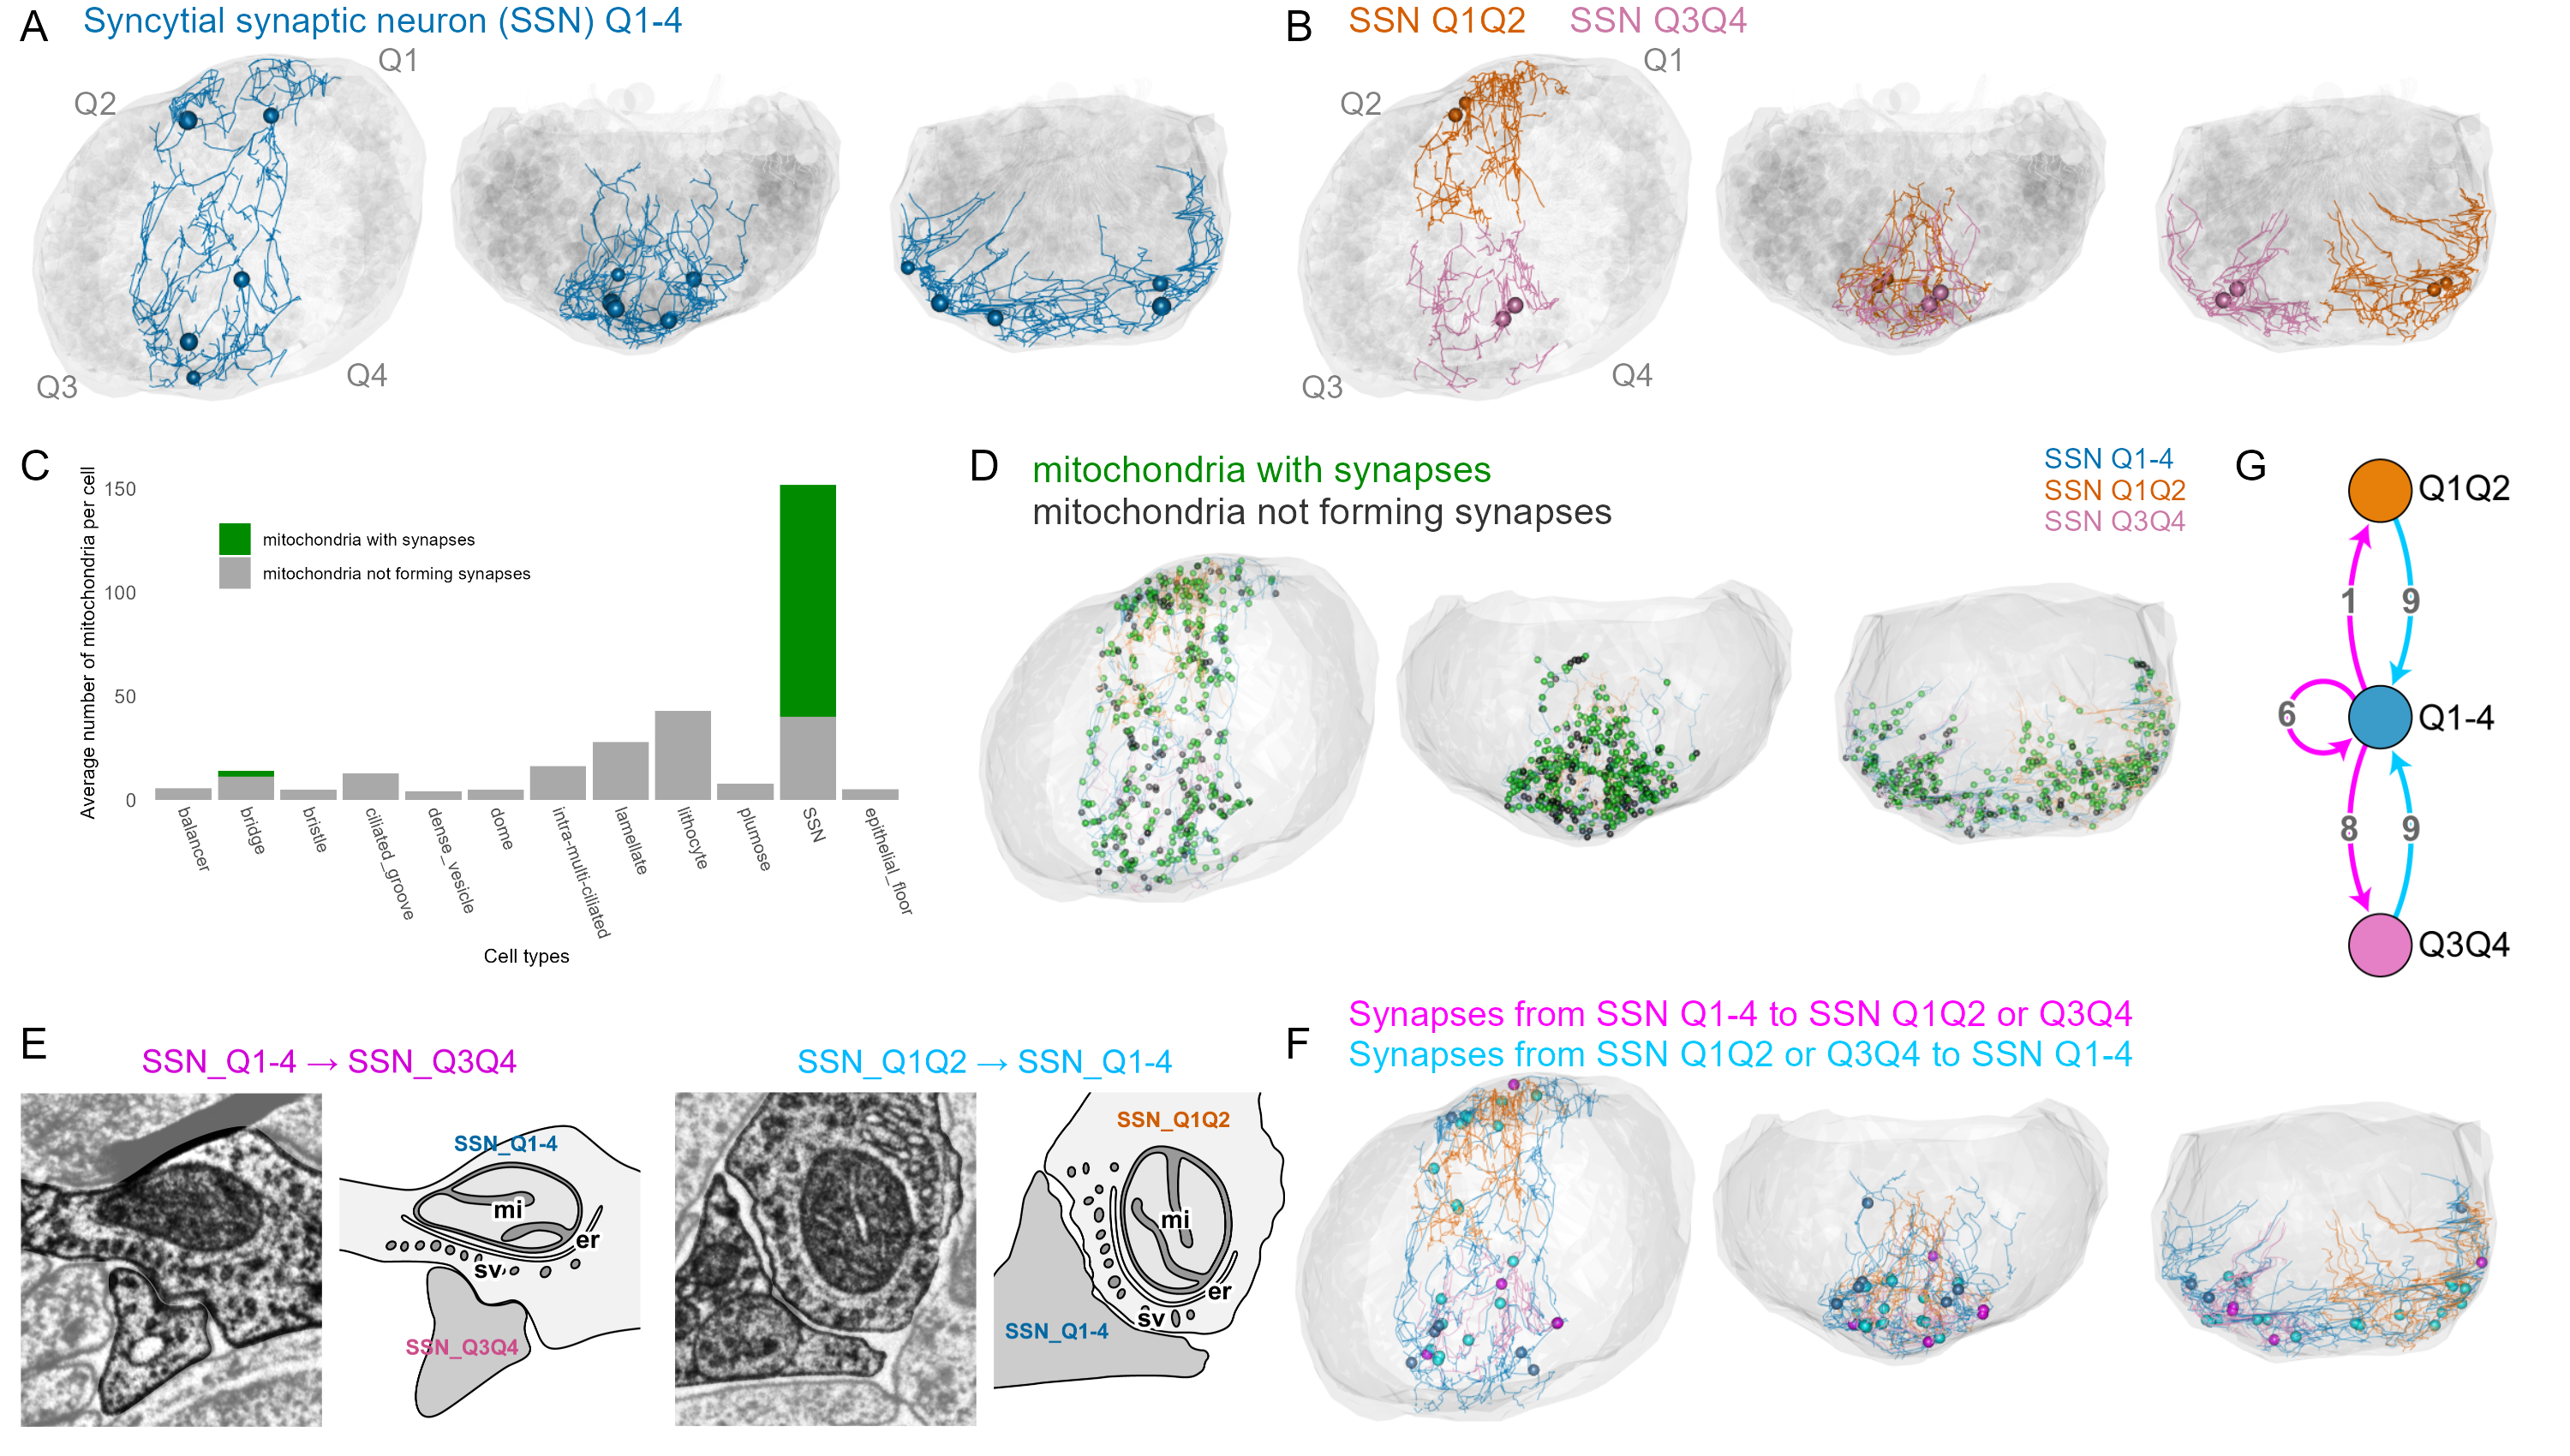
\includegraphics[width=1\textwidth,height=\textheight]{figures/Figure2.png}

}

\caption{\textbf{Figure 2. Title fig 2} pic of a larva, boxed region of
AO, schematic, catmaid pic with slice, dimensions, quadrants, regions,
(A) legend (B) legend.}

\end{figure}%

\subsubsection{Identification the Gravity-Sensitive Neural Circuit via
the Syncytial Neurons
Network}\label{identification-the-gravity-sensitive-neural-circuit-via-the-syncytial-neurons-network}

We discovered that AO neurons form synaptic connections with each other,
and that AO neuron\_Q1234 forms self-synapses, or ``autapses.'' To our
knowledge, previous reports have not identified synaptic connections
between subepithelial nerve net (SNN) neurons. Thus, our results
represent the first report of synaptic connectivity between neurons in
the apical organ, forming a network in ctenophores (subject to
confirmation). These AO neuron networks were found to form many
presynaptic structures in relation to the gravity-sensing balancer
cells.

Balancer cells are monociliated cells, and their cilia protrude longer
than those of other monociliated cells. Moreover, the cilia of balancer
cells are bundled into four groups at the center of the apical organ,
forming a compound cilium. Based on these features, we identified and
classified the balancer cells. The cellular arrangement differed clearly
when viewed in the lateral view, sagittal plane, and tentacular plane,
with the cell bodies gathering toward the apical organ in the tentacular
plane. In each quadrant, the number of cells was as follows: Q1: 37, Q2:
32, Q3: 32, Q4: 28. Each cell contained 3 to 10 ? mitochondria.

From AO neuron\_Q1Q2, synapses were formed with 6 of the 37 balancer
cells in the Q1 region, and 8 of the 32 balancer cells in the Q2 region.
Similarly, from AO neuron\_Q3Q4, synapses were formed with 1 of the 32
balancer cells in the Q3 region, and 5 of the 28 balancer cells in the
Q4 region. AO neuron\_Q1234 formed input synapses with balancer cells in
the Q1 region (7 cells), Q2 region (11 cells), Q3 region (6 cells), and
Q4 region (10 cells). Some balancer cells received inputs from both AO
neuron\_Q1Q2 or AO neuron\_Q3Q4 and AO neuron\_Q1234. While previous
studies have suggested the presence of afferent synapses from balancer
cells to neurons (\textbf{Hernandez\_Nicaise\_1974?}), our data did not
reveal any synaptic inputs from balancer cells to AO neurons. However,
we identified ``bridge cells'' that actively formed input synapses with
AO neurons, highlighting their potential role in the network.

\begin{figure}[H]

{\centering 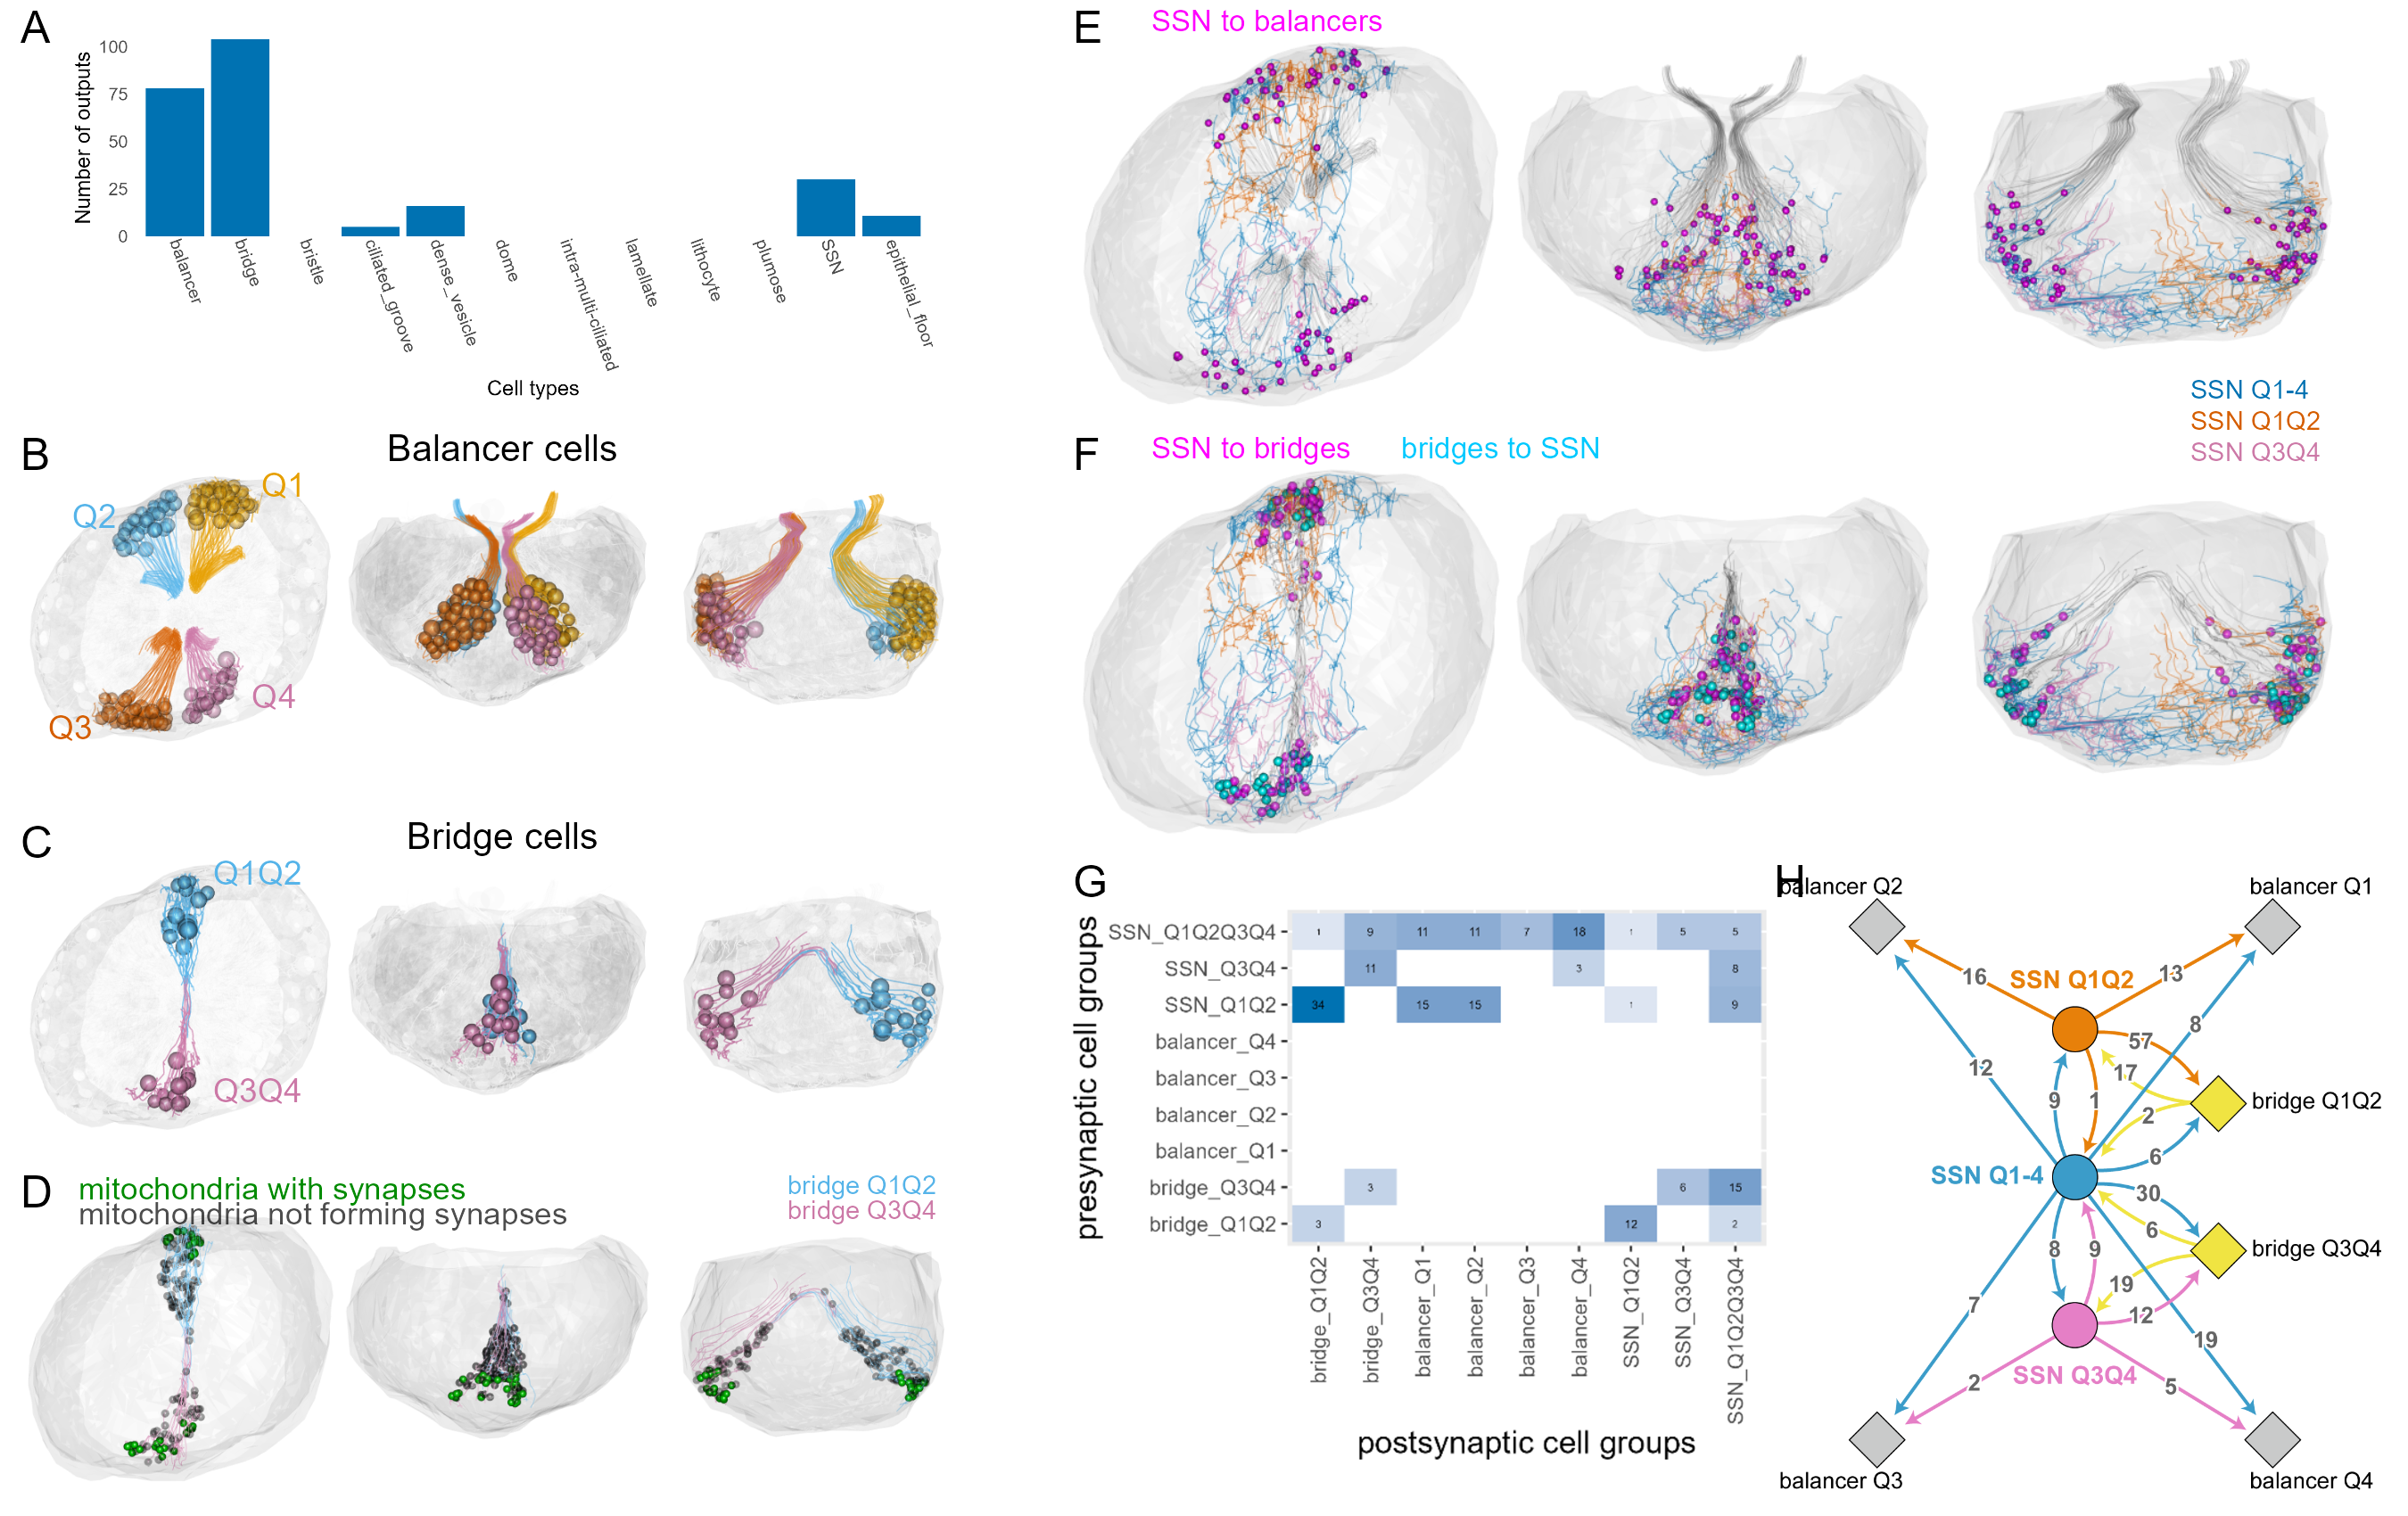
\includegraphics[width=1\textwidth,height=\textheight]{figures/Figure3.png}

}

\caption{\textbf{Figure 3. Title fig 3} pic of a larva, boxed region of
AO, schematic, catmaid pic with slice, dimensions, quadrants, regions,
(A) legend (B) legend.}

\end{figure}%

\subsubsection{Identification of Neuron-like Bridge Cells Forming
Afferent Synapses in the Gravity-Sensitive Neural
Circuit}\label{identification-of-neuron-like-bridge-cells-forming-afferent-synapses-in-the-gravity-sensitive-neural-circuit}

From our data, we identified several cell groups that form multiple
afferent synapses with AO neurons. These cells, based on their
morphological features, were found to be the bridge cells first
described by Tamm et al.~in 2002 (\textbf{Tamm\_and\_Tamm\_2002?}).
These cells are characterized by bundles of elongated processes filled
with microtubules that arch over the epithelial layer, resembling a
bridge. They originate from the base of paired balancer cells along the
tentacle surface and extend across the sagittal plane toward the base of
the opposite balancer cells. In regions where the mitochondria of the
bridge cells are localized (approximately 30\%), a presynaptic triad
structure, similar to that of AO neurons, was found, containing synaptic
vesicles and smooth endoplasmic reticulum.

Our three-dimensional reconstruction data revealed that the bridge cells
form two distinct cell groups across the sagittal plane, between the
Q1Q2 and Q3Q4 regions. In the Q1Q2 region, 14 cells were identified,
while in the Q3Q4 region, 12 cells were identified, totaling 26 bridge
cells. Nearly all of these bridge cells (25 out of 26) exhibited
afferent synapses from AO neurons. For bridge cells located in the Q1Q2
region, synaptic inputs came primarily from AO neuron\_Q1Q2 (11 cells),
AO neuron\_Q1234 (1 cell), or both (2 cells). For bridge cells located
in the Q3Q4 region, synaptic inputs were received from AO neuron\_Q3Q4
(1 cell), AO neuron\_Q1234 (7 cells), or both (1 cell). In other words,
bridge cells in the Q1Q2 region mainly received input from AO
neuron\_Q1Q2, while those in the Q3Q4 region received input primarily
from AO neuron\_Q1234, showing a distinct pattern of input in the two
regions.

Some bridge cells also formed afferent synapses with AO neurons. For
example, bridge cells in the Q1Q2 region formed synapses with AO
neuron\_Q1Q2 (3 cells) or both AO neuron\_Q1Q2 and AO neuron\_Q1234 (2
cells). Bridge cells in the Q3Q4 region formed synapses with AO
neuron\_Q3Q4 (1 cell) or AO neuron\_Q1234 (6 cells). A notable
difference was observed between the Q1Q2 and Q3Q4 regions in the
proportion of synaptic inputs from bridge cells to AO neurons.

Interestingly, in both regions, bridge cells also formed synapses with
adjacent bridge cells. However, no synaptic input was found from bridge
cells across the sagittal plane to those in the opposite region. To
analyze the grouped synaptic connectivity graph, we classified cell
types within each region, collapsed cells of the same type into a single
node, summed the number of synapses, and explored directed pathways to
effectors (balancer cell groups). The results revealed a feedback
pathway from AO neurons through the synaptic connections formed by
bridge cells, thereby shedding light on the neural circuit structure
involving these cells.

\begin{figure}[H]

{\centering 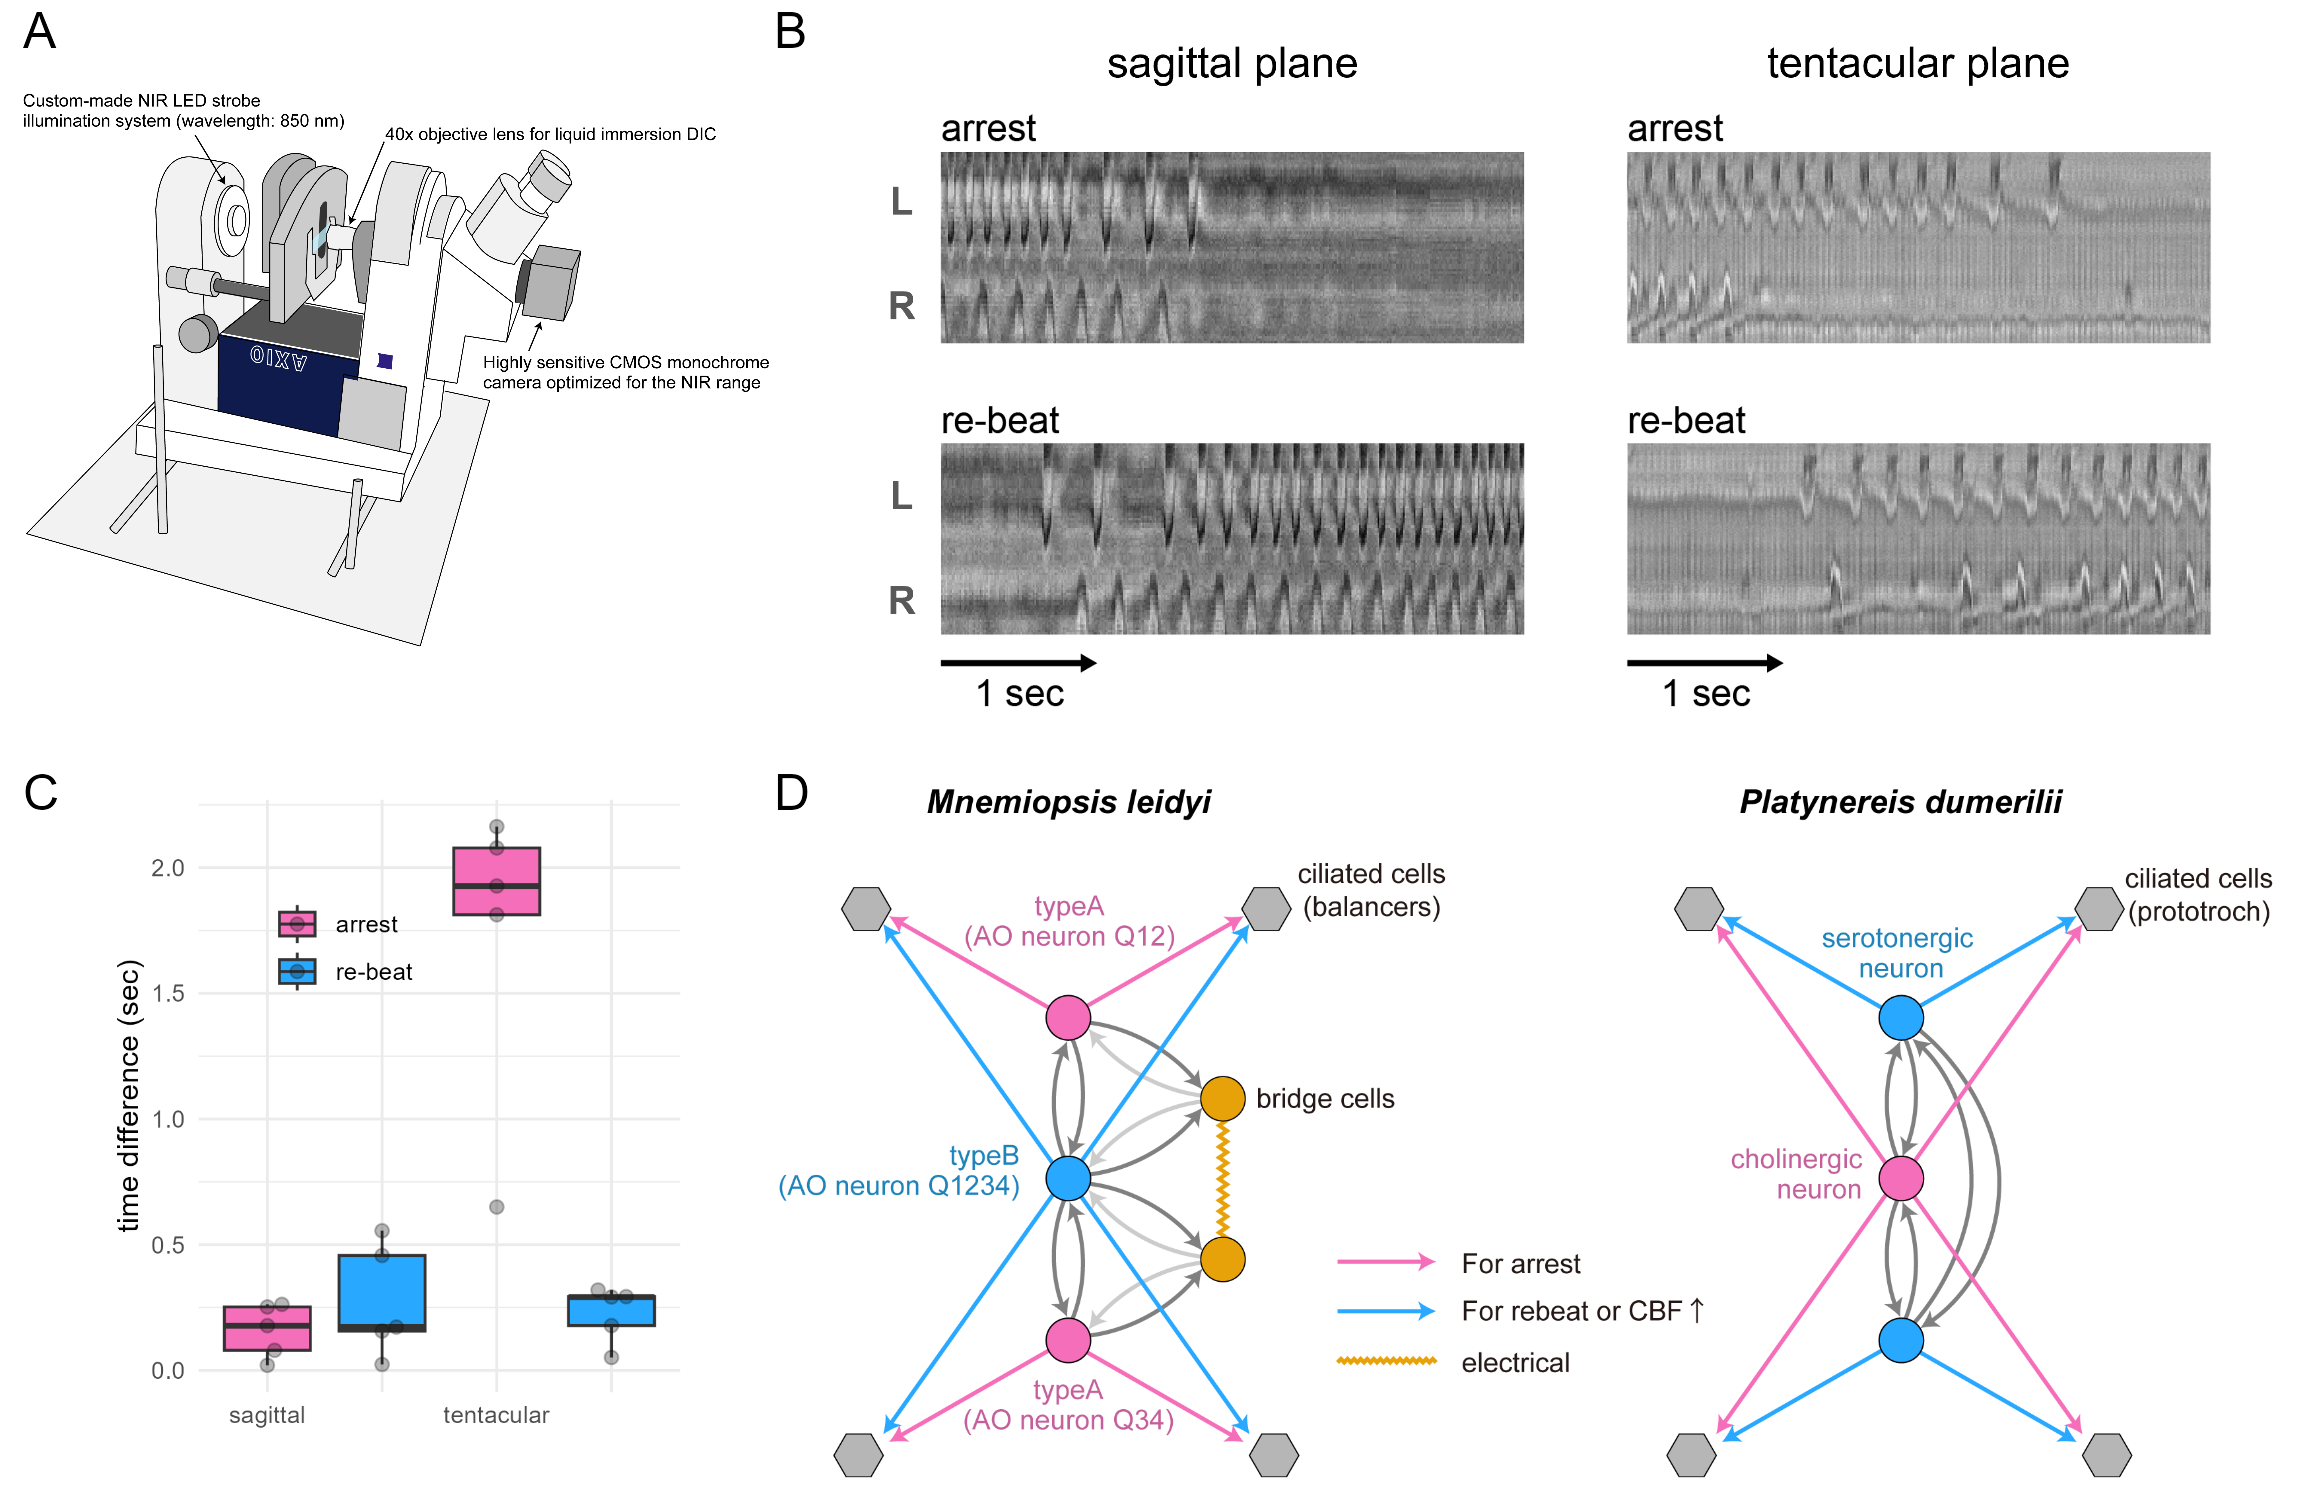
\includegraphics[width=1\textwidth,height=\textheight]{figures/Figure4.png}

}

\caption{\textbf{Figure 4. Title fig 4} pic of a larva, boxed region of
AO, schematic, catmaid pic with slice, dimensions, quadrants, regions,
(A) legend (B) legend.}

\end{figure}%

\subsubsection{Control of Balancer Ciliary Movements by
Gravity-Sensitive Neural
Circuits}\label{control-of-balancer-ciliary-movements-by-gravity-sensitive-neural-circuits}

To investigate the function of gravity-sensitive circuits, we conducted
a comparative analysis of balancer ciliary movements across different
regions. Previous studies (Tamm, 1980, 1982; Lowe, 1997) have
established that balancer cilia function as mechanoreceptors, with their
beating frequency modulated by inclination. Furthermore, it has been
suggested that differences in the asymmetry of statolith morphology and
the elongation direction of balancer cilia between the tentacular and
sagittal planes could result in variations in the force received from
the statolith (Tamm, 2014, 2015). Building on these findings, we
standardized conditions for observing balancer cilia by tilting the
microscope by 90 degrees and fixing samples such that the aboral-oral
axis was aligned parallel to the vertical stage, with the aboral side
facing upward. Using connectome analysis, we aimed to evaluate the
neural circuit differences by analyzing the control patterns of left and
right balancer cilia in the tentacular and sagittal planes.
Specifically, we hypothesized that differences in control between Q1
(Q2) and Q3 (Q4) regions, as well as between Q1 (Q4) and Q2 (Q3)
regions, would reveal distinct functions of AO neurons (e.g., AO neuron
Q12/Q34 vs.~AO neuron Q1234). For the sagittal plane, we recorded
balancer ciliary movements in the Q1(4) and Q2(3) regions (left and
right sides of the image) and, for the tentacular plane, in the Q1(3)
and Q2(4) regions, using a high-speed camera (100 fps) for 2 minutes
(12,000 frames). Regions of interest (ROIs) were defined in areas where
brightness changes indicated ciliary beating. We measured these
brightness changes to generate dynamics graphs of balancer ciliary
movements for both planes.

During the 2-minute recordings, balancer cilia exhibited movements that
could be fast, slow, or stop abruptly (arrest) and start moving again
(re-beat). Occasionally, large contraction responses caused the entire
cydippid to move out of frame, and data from these moments were
excluded. We focused on two metrics for left-right comparison: (1) the
timing of ciliary arrest and (2) the timing of re-beat initiation
following an arrest. Due to the low baseline beating frequency of the
cilia, rapid synaptic input responses were not evaluated, suggesting
that ciliary beat regulation may involve non-synaptic control
mechanisms. The analysis revealed that both arrest and re-beat events
were synchronized between left and right balancers in both planes within
a few milliseconds, suggesting that these events are governed by
synaptic input from neurons. Interestingly, while the re-beat timing
showed no significant differences between the sagittal and tentacular
planes, arrest timing exhibited greater variability in the tentacular
plane. Comparing these findings with neural circuit diagrams suggests
that in the sagittal plane, the same AO neurons (Q12 or Q34) project to
both balancer cell groups, transmitting signals simultaneously and
enabling synchronization. In contrast, in the tentacular plane, separate
AO neurons project to different regions, potentially introducing an
additional synaptic step, which may account for the observed variability
in arrest timing.

\begin{figure}[H]

{\centering 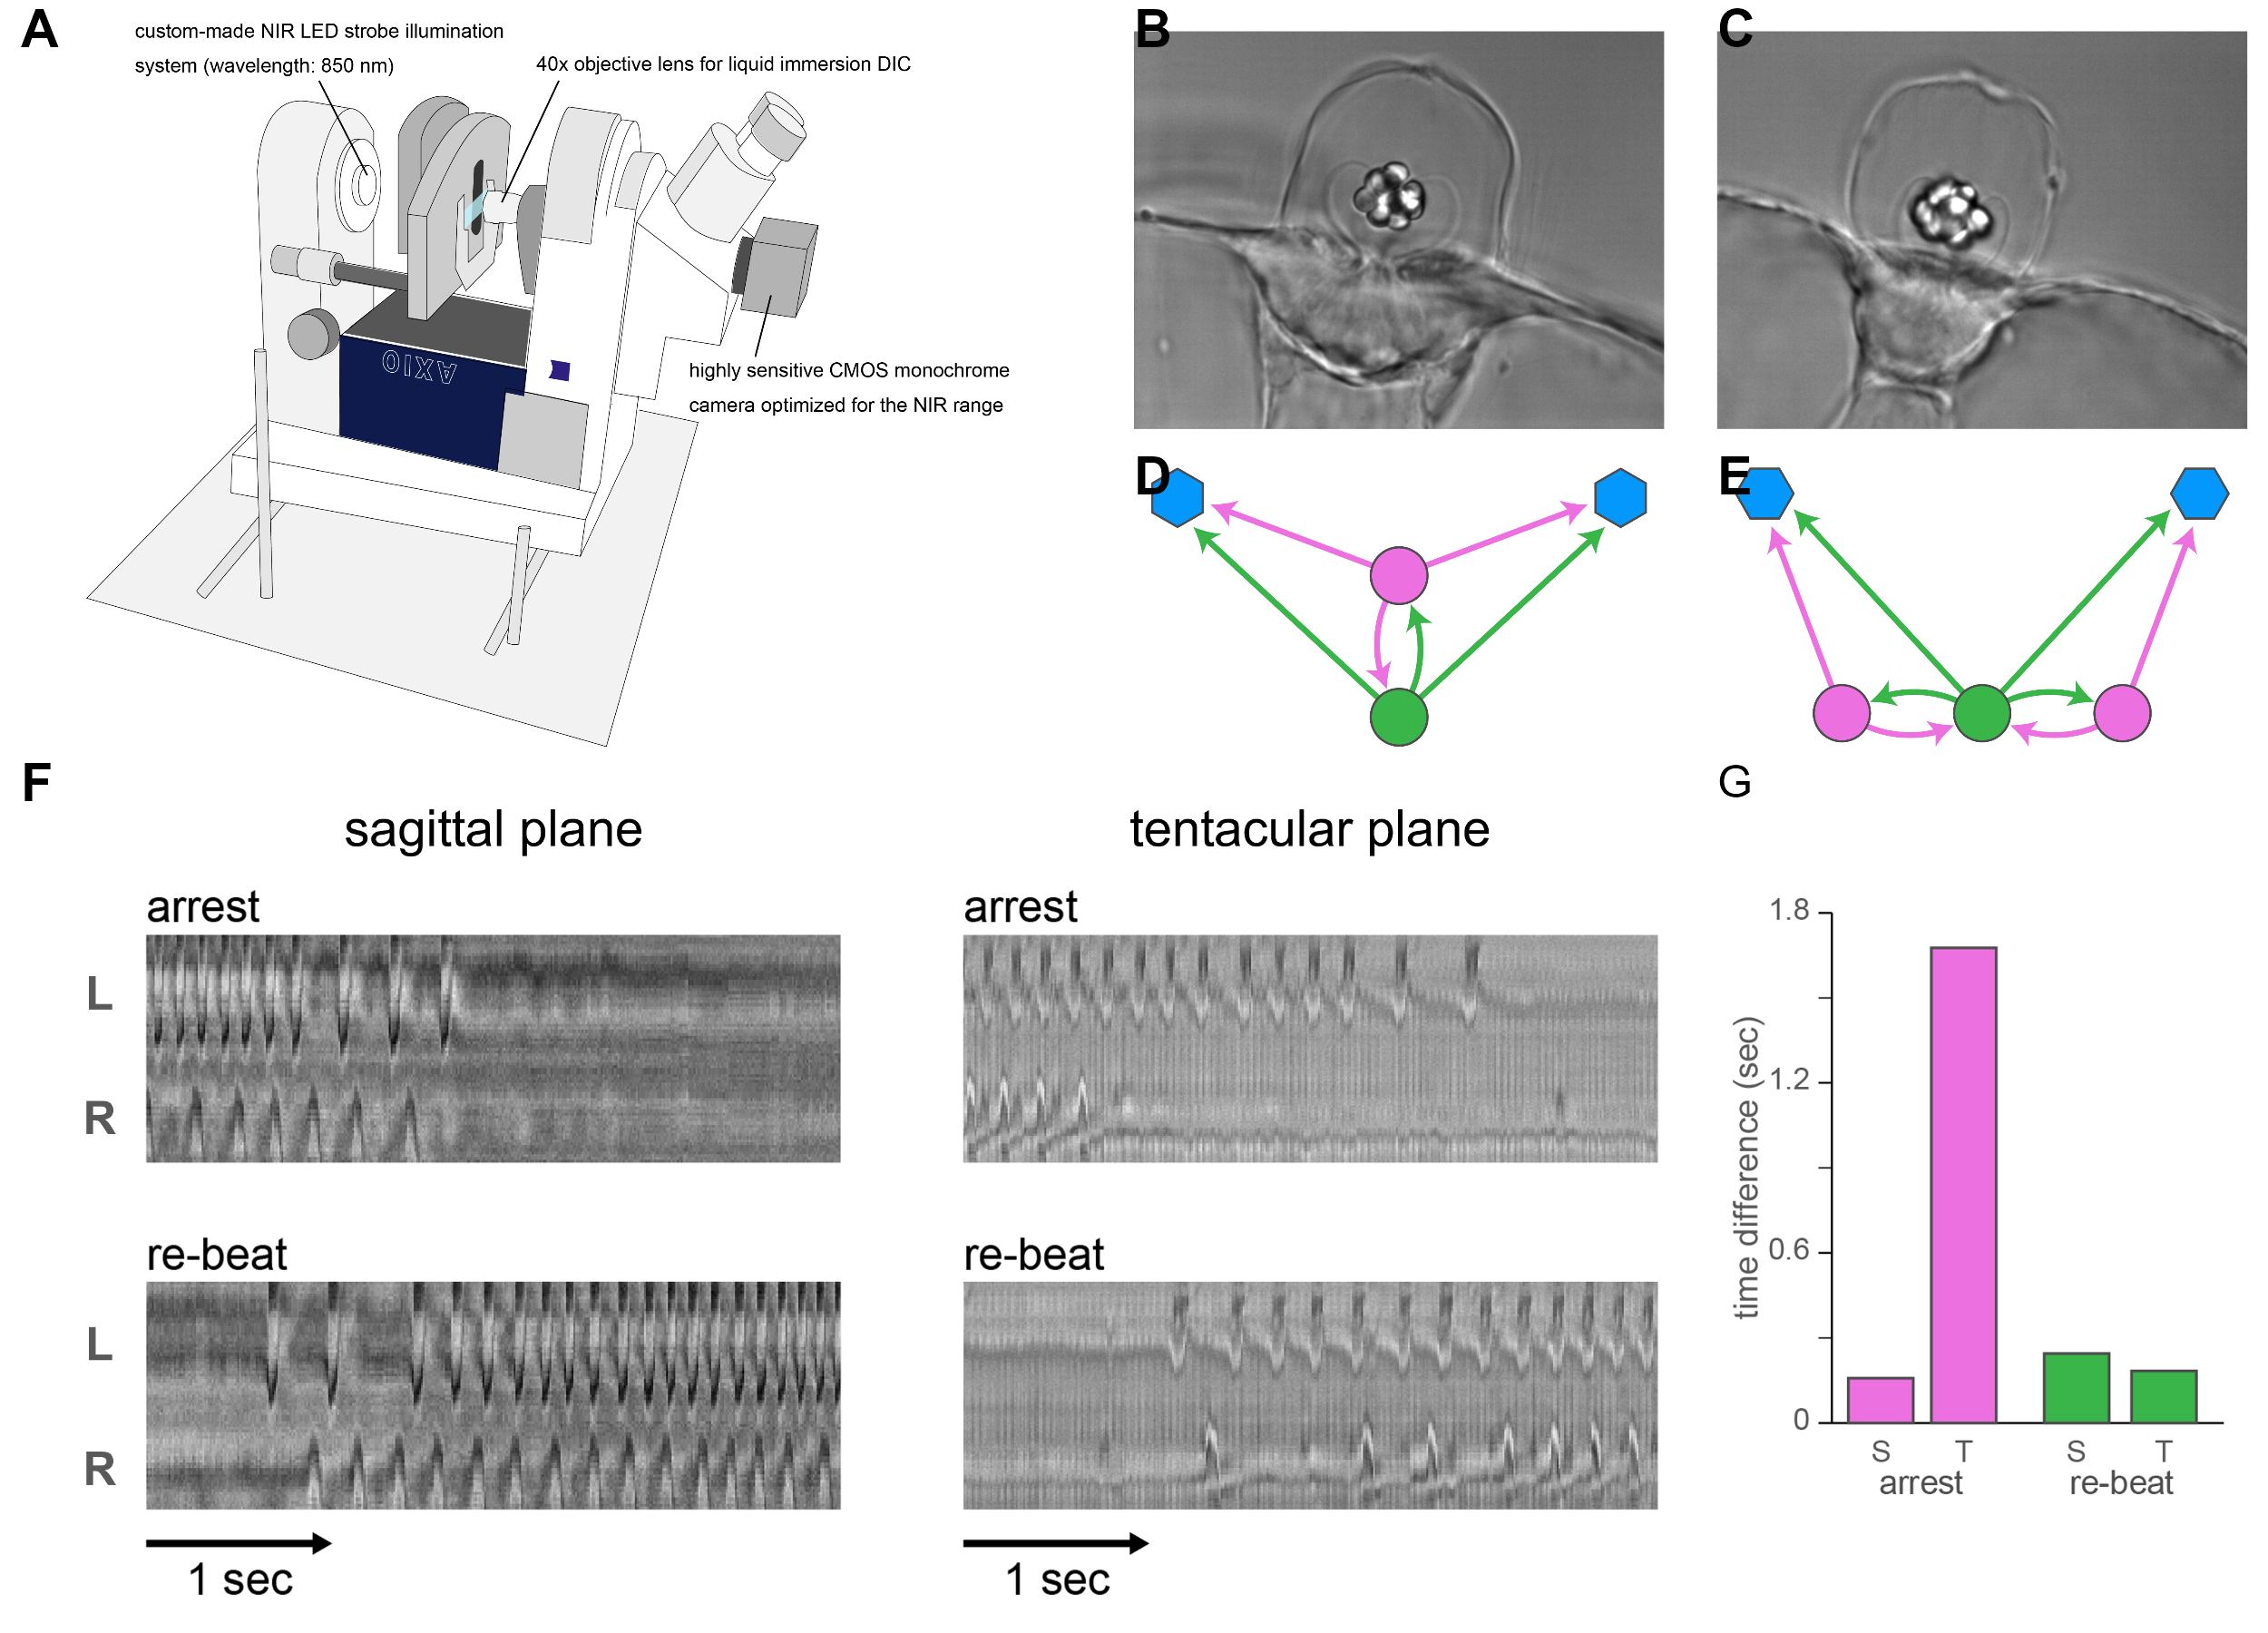
\includegraphics[width=1\textwidth,height=\textheight]{figures/Figure5.png}

}

\caption{\textbf{Figure 5. Title fig 5} pic of a larva, boxed region of
AO, schematic, catmaid pic with slice, dimensions, quadrants, regions,
(A) legend (B) legend.}

\end{figure}%

\subsection{Discussion}\label{discussion}

In this study, we traced all the constituent cells of the aboral organ
in five-day-old larvae of \emph{Mnemiopsis leidyi} and completed a
comprehensive neural map. As a result, we identified a novel type of
syncytial neuron with a previously unreported morphology. Furthermore,
we found that three such syncytial neurons project to distinct
quadrants, integrating with balancer cell groups to form a
gravity-sensing neural circuit. This study represents the first complete
neural circuit map reported in ctenophores. Additionally, our analysis
of balancer ciliary movements, based on neural circuit data, revealed
differences in ciliary arrest control arising from circuit variations.

\subsubsection{Identification of a Previously Unreported Syncytial
Neuron}\label{identification-of-a-previously-unreported-syncytial-neuron}

We identified three syncytial neurons with multiple nuclei in the apical
organ of five-day-old \emph{M. leidyi} cydippid larvae. Burkhurdt et
al.~(2023) previously reported that in one-day-old larvae, the
sub-epithelial nerve net (SNN) contains neurons that form syncytia.
However, the newly discovered syncytial neurons embedded within the
apical organ cell cluster did not exhibit the characteristic ``pearl
necklace-like structure'' of the SNN, which consists of microtubules
connecting neurons. Instead, their morphology was more reminiscent of
fiber cells previously described in Placozoa (Mayorova et al., 2021),
with cell bodies extending through intercellular spaces. These
morphological characteristics suggest that the newly identified neurons
represent a second distinct type of syncytial neuron in ctenophores.

\subsubsection{Functional Diversification of the Three Syncytial
Neurons}\label{functional-diversification-of-the-three-syncytial-neurons}

The three identified neurons may be classified into two distinct
functional types based on their spatial arrangement and their influence
on the differential control of balancer ciliary movement between the
quadrants. In metazoans, a single neuron can directly provide synaptic
input to multiple ciliated cells at a distance, synchronizing their
movements. For instance, in larvae of the annelid \emph{Platynereis
dumerilii}, a cholinergic motor neuron (MC) innervates multiple
prototroch ciliated cells, synchronizing their motion such that
activation of the neuron leads to simultaneous arrest of ciliary beating
(Verasztó et al., 2017). Additionally, a pair of serotonergic neurons,
designated Ser-h1, extend axons that cross at the midline; the left
Ser-h1\_l predominantly innervates right-sided ciliated cells, while the
right Ser-h1\_r mainly projects to the left-side ciliated cells.
Activation of Ser-h1 induces ciliary beating initiation and increases
beat frequency.

In the this study, we found that three neurons are closely positioned
within the confined space of the apical organ, potentially enabling a
single neuron to control distant ciliary movements in a synchronized
manner. Moreover, the presence of neurons projecting to the same
ciliated cells in distinct patterns suggests that these neurons may
serve opposing functions---one inhibiting ciliary activity while the
other promotes it, or one modulating ciliary beat frequency. While our
synaptic ultrastructure analysis did not allow us to distinguish
excitatory from inhibitory neurons, future electrophysiological
investigations will be essential to elucidate their functional
properties.

\begin{figure}[H]

{\centering 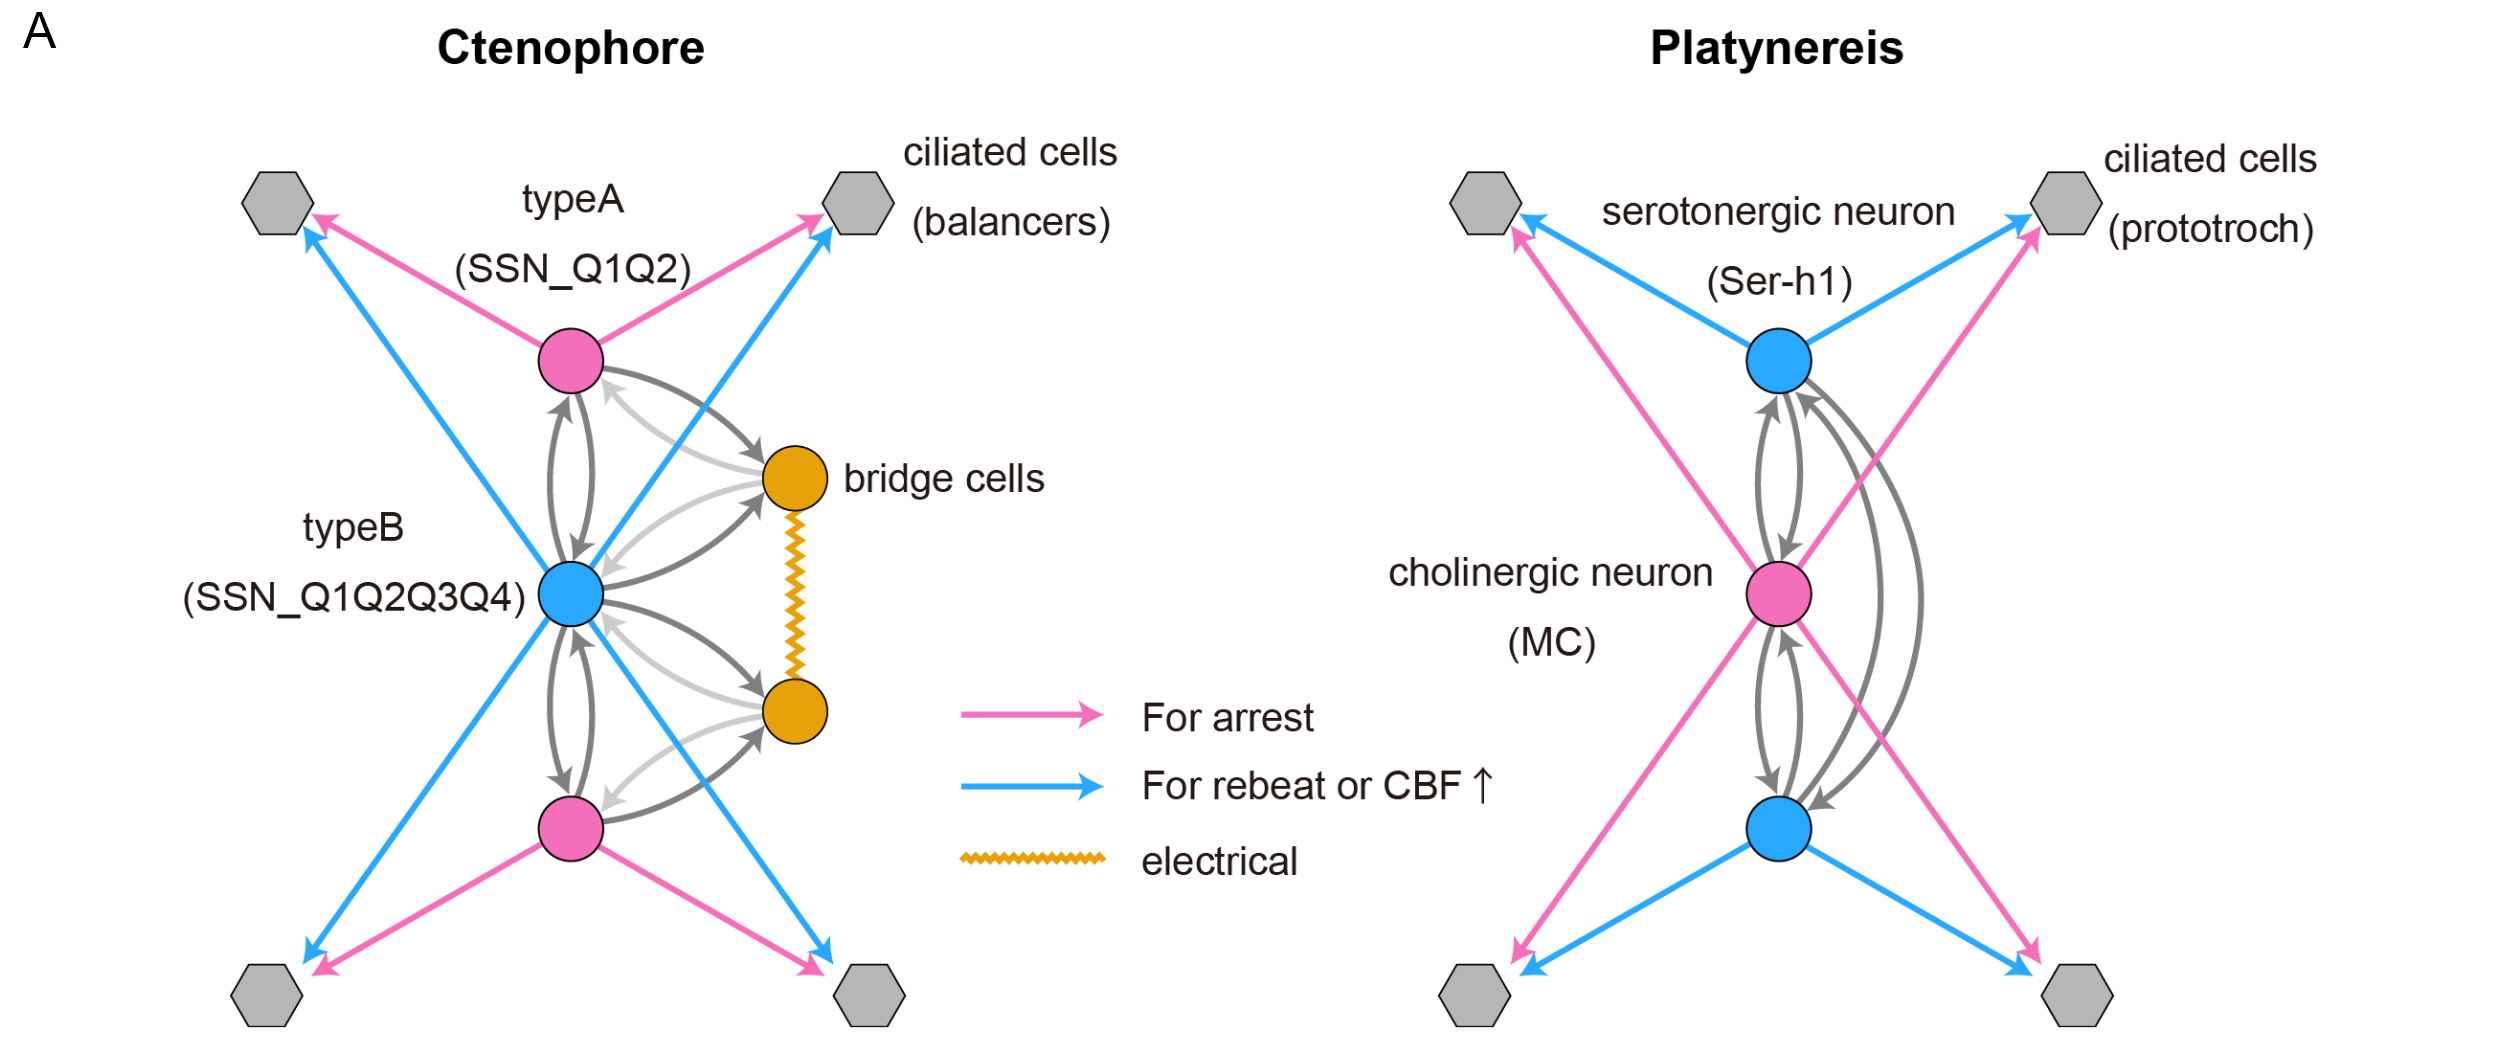
\includegraphics[width=1\textwidth,height=\textheight]{figures/Figure6.png}

}

\caption{\textbf{Figure 6. Title fig 6} pic of a larva, boxed region of
AO, schematic, catmaid pic with slice, dimensions, quadrants, regions,
(A) legend (B) legend.}

\end{figure}%

\subsubsection{Paracrine Signaling and Synaptic Transmission from
Sensory to Neural
Cells}\label{paracrine-signaling-and-synaptic-transmission-from-sensory-to-neural-cells}

Previous electron microscopy studies have suggested the presence of
various sensory cells, including photoreceptor and mechanoreceptor
cells, within the aboral organ of ctenophores (Horridge, 1965; Krisch,
1973; Aronova, 1974; Vinnikov, 1974). By comparing our dataset with
previously reported ultrastructural data, we successfully identified
several sensory cells within the apical organ. However, notably, we did
not find any clear presynaptic structures between these sensory cells
and either neural or other cellular targets. In prior studies,
immunostaining for specific neuropeptides in ctenophores has revealed
positive signals in distinct cell populations within the apical organ
(Sachkova et al., 2021; Hayakawa et al., 2022). These findings suggest
that many sensory cells in the apical organ may primarily rely on
neuropeptide-mediated paracrine signaling rather than direct synaptic
connections, supporting the chemical brain hypothesis (Jekely, 2021).
While paracrine transmission is generally slower than synaptic
transmission, it allows for a greater diversity of information
processing.

Conversely, previous research has demonstrated that mechanoreceptive
sensory cells equipped with cilia (referred to as type 3 and type 4
cells) in ctenophores form direct synaptic connections with the
sub-epithelial nerve net (SNN) and mesogleal neurons (Burkhurdt et al.,
2023). Based on their ultrastructural features, these sensory cells are
believed to respond to physical stimuli such as water flow, vibrations,
and direct contact, transmitting information rapidly to cilia and muscle
cells (Hertwig, 1880; Chun, 1880; Eimer, 1880).

Surprisingly, our study identified bridge cells as the primary cell type
forming synaptic inputs onto neurons in the apical organ. Bridge cells
were first described by Tamm et al.~(2002) based on their morphological
characteristics, with cellular projections extending to the basal region
of balancer cilia (Tamm \& Tamm, 2002). Our findings suggest that bridge
cells are electrically coupled to balancer cilia and provide rapid
feedback to neurons via synaptic transmission. Future studies analyzing
differential responses to various sensory stimuli will not only
elucidate the functional roles of bridge cells but also provide insights
into the evolutionary relationship between transmission speed and
synapse development.

\subsubsection{Circuit Variability as a Driver of Behavioral
Diversity}\label{circuit-variability-as-a-driver-of-behavioral-diversity}

Our study suggests that differences in neural circuits contribute to
variations in the timing of ciliary arrest, which may play a role in
modulating swimming direction in ctenophores (Richard Satterlie, 2015).
This finding provides evidence that increased circuit complexity
contributes to behavioral diversification. By integrating multiple
neurons and altering circuit structure, information can be branched,
allowing for diverse motor patterns within the framework of fast
synaptic transmission.

The neural cells identified in the apical organ exhibit a divergent
feedforward connectivity pattern, where a single neuron forms
presynaptic connections with multiple downstream targets. Such a circuit
design minimizes unwanted signal interference, reduces processing
delays, and enables relatively fast response execution (Luo, 2021).
Moreover, the presence of multiple divergent feedforward circuits
suggests that slight variations in the synchronization and phase delay
of ciliary beating (within the range of a few hundred milliseconds) may
have evolved as a mechanism for generating behavioral diversity.

From a broader neuroanatomical perspective, nervous system structures
across various animals have been shaped through selective optimization
to adapt to environmental constraints (Bullmore \& Sporns, 2012; Perin
et al., 2011). For example, in nematodes, the spatial arrangement of
ganglia is optimized to minimize the total length of neural wiring
(White et al., 1986). Similarly, in ctenophores, understanding how
transmission via syncytial neurons and synaptic connections has been
selectively optimized at the circuit level will provide crucial insights
into the evolutionary scaling of neural networks from early nervous
systems to complex brains (Farnworth and Montgomery, 2024). In
particular, this research may help elucidate how circuit modularization
and layered structures emerged over evolutionary time.

\subsection{Materials and Methods}\label{materials-and-methods}

\subsubsection{Data and Code
Availability}\label{data-and-code-availability}

The following EM image stacks, including all traces and annotations, are
available at https://catmaid.jekelylab.ex.ac.uk. These datasets can be
queried either within CATMAID or through the CATMAID application
programming interface (API) using the catmaid or natverse packages
(Bates et al., 2020). The dataset encompasses all EM images (in JPG
format), skeletons, meshes, node tags, connectors, and annotations.
Additionally, we provide all R scripts used for data acquisition and
figure generation (Jokura et al., 2025). All plots, figures (including
anatomical renderings), and figure layouts can be fully reproduced using
the provided R scripts. While the scripts are mostly organized by
figure, some general-purpose scripts---for tasks such as loading
libraries, accessing CATMAID data, and defining common functions---are
shared across multiple figures.

\subsubsection{Specimen Preparation, Transmission Electron Microscopy,
and Image
Processing}\label{specimen-preparation-transmission-electron-microscopy-and-image-processing}

Larvae of Mnemiopsis leidyi (5 days old) were cryofixed using a
high-pressure freezing apparatus (BAL-TEC HPM 010, Balzers) and
immediately transferred to liquid nitrogen for storage. The frozen
samples were processed in a substitution medium containing 2\% (w/v)
osmium tetroxide and 0.5\% uranyl acetate in acetone, using a
cryo-substitution device (EM AFS-2, Leica). Cryo-substitution was
performed by gradually raising the temperature, and the samples were
embedded in epoxy resin. Serial sections of 50 nm thickness were
prepared using a Reichert Jung Ultracut E ultramicrotome and a 45º
DiATOME diamond knife. To enhance section adhesion and improve
hydrophilicity, a conductive indium tin oxide-coated glass slide (ITO
Glass, UQG Optics) was treated with air glow discharge using the PELCO
easiGlow system (Ted Pella, Inc.), rendering the carbon film surface
negatively charged. Section ribbons were collected on the prepared glass
slides, slowly dried to ensure proper stretching, and firmly adhered to
the glass surface. The sections on glass were stained with UranyLess and
lead citrate (Reynolds) using airless staining bottles (Delta
Microscopies). The glass slides were mounted on STEM-specific stages
(Zeiss) using Copper Foil EMI Shielding Tape (3M). Imaging was performed
using a Gemini SEM 500 (Zeiss) equipped with SmartSEM and Atlas 5
imaging software (Zeiss). The full dataset consisted of 620 serial
sections, each 50 nm thick. The imaging resolution was 2.8 nm/pixel,
using electron holography transmission at an acceleration voltage of 1.5
kV (in-lens detector, dwell time: 3 µs).

\subsubsection{Image-Stack Realignment and Spatial Data Transformation
in
CATMAID}\label{image-stack-realignment-and-spatial-data-transformation-in-catmaid}

To process the image stack, we utilized the TrakEM2 plugin of FIJI
(ImageJ) (version 2.0.0-rc-15/1.49k / Java 1.6.0\_24 (64-bit) -- 2014).
A project was created, and all TIFF images were imported using the
``import sequence as grid'' function. Subsequently, the following
filters were applied sequentially: Invert, Equalize Histogram, and
Gaussian Blur.

The alignment process consisted of three stages, each progressively
refining the spatial accuracy:

Rigid Alignment Initially, a rigid alignment was performed with the
following parameters: least squares mode (linear feature
correspondences), encompassing the entire layer range with the first
layer as the reference. Only visible images were used, without
propagation. The alignment was executed with an initial Gaussian blur of
1.6 pixels, three steps per scale octave, a minimum image size of 512
pixels, and a maximum of 2048 pixels. Additional parameters included a
feature descriptor size of 8, orientation bins of 8, and a closest ratio
of 0.92. The alignment allowed clearing the cache, using 32 feature
extraction threads, a maximal alignment error of 100 pixels, a minimal
inlier ratio of 0.20, and a minimum of 12 inliers. The expected and
desired transformations were set to rigid, with testing multiple
hypotheses (tolerance: 5.00 pixels) and considering up to 5 neighboring
layers, giving up after 5 failures. Regularization was performed with a
maximal iteration of 1000, a maximal plateau width of 200, and a rigid
lambda of 0.10.

Affine Alignment Following the rigid alignment, an affine alignment was
applied using similar parameters, except the expected and desired
transformations were set to affine. The minimal image size was reduced
to 64 pixels, while the other parameters (e.g., Gaussian blur, feature
descriptor size, inliers, and testing hypotheses) remained unchanged to
ensure consistent processing.

Elastic Alignment Two iterations of elastic alignment were performed to
fine-tune the spatial data. Key parameters included a block matching
layer scale of 0.05, a search radius of 200 pixels, a block radius of
2000 pixels, and a resolution of 60. Correlation filters were employed
with a minimal PMCC r of 0.10, a maximal curvature ratio of 1000, and a
maximal second-best r/best r of 0.90. A local smoothness filter was
applied with the approximate local transformation set to affine, a local
region sigma of 1000 pixels, and an absolute maximal local displacement
of 10 pixels (relative maximal displacement: 3.00). Pre-aligned layers
were tested for up to 4 neighboring layers. The elastic alignment used a
rigid approximation, maximal iterations of 3000, a plateau width of 200,
spring mesh stiffness of 0.01, and a maximal stretch of 2000 pixels. A
legacy optimizer was employed to enhance performance.

After each alignment stage, the project was saved as an XML file under a
unique name to preserve iterative progress. Finally, the images were
exported from FIJI using TrakEM2 in a format compatible with CATMAID.

\subsubsection{Neuron Tracing, Synapse Annotation, and
Review}\label{neuron-tracing-synapse-annotation-and-review}

The reconstruction of cells and connectivity was performed using CATMAID
(Saalfeld et al., 2009), analyzing a total of 620 serial sections. To
digitally reconstruct all neurons within the serial TEM dataset, we
utilized the collaborative web-based application CATMAID, installed on a
local server (Saalfeld et al., 2009; Schneider-Mizell et al., 2016). To
mark the locations of cell bodies, we placed tags at the approximate
center of each nucleus within the dataset. At each nuclear center, the
radius of the single node was adjusted according to the size of the cell
body in that specific layer. All skeletons were rooted at their
respective cell bodies, and nodes were tagged as ``soma.'' Synapses were
identified based on four key structural features: the cell membrane,
synaptic vesicles, the endoplasmic reticulum, and mitochondria. Most
synapses could be verified across consecutive sections, ensuring
accurate annotation and connectivity mapping.

\subsubsection{Cell Nomenclature and
Annotations}\label{cell-nomenclature-and-annotations}

Each cell is assigned a specific type name based on its category
(balancer, biC, bridge, bristle, dense vesicle cell, dome, EF, IcMC, LB,
lithocyte, monoC, non-C, plumose cell, SNN, ssCG, SSN, stCG), resulting
in a total of 17 cell types. Additionally, a quadrant number is appended
to the cell type name following an underscore (``\_'') to indicate the
cell body's location. For example, cells located in the first quadrant
are annotated with ``Q1.'' If a cell is situated between the first and
second quadrants, the annotation ``Q1Q2'' is applied.

Cells of the same type within the same region are further distinguished
by serial numbering. Each cell is also assigned multiple annotations,
which can be utilized to query the database via CATMAID or the CATMAID
API (e.g., using the R catmaid package). These annotations provide a
structured and precise framework for identifying and analyzing specific
cells, facilitating robust data integration and retrieval within the
dataset.

This system ensures consistent and accurate tracking of cellular data,
enabling comprehensive analysis of cellular structures and functions
across regions.

\subsubsection{Analysis of Balancer
Cilia}\label{analysis-of-balancer-cilia}

We conducted the analysis using the cydippid stage of Mnemiopsis leidyi
at five days post-fertilization. A coverslip with a thin layer of
Vaseline applied to two edges was lightly placed on a slide glass.
Filtered natural seawater was introduced under the coverslip, along with
the cydippids. By gently moving the coverslip, the desired orientation
for observation was adjusted, and once positioned, slight pressure was
applied to immobilize the cydippids. To stabilize the statolith's
position, the microscope was tilted 90 degrees, arranging the stage
vertically. The movement of the balancer cilia was observed using a
differential interference contrast (DIC) microscope (Zeiss Axio
Imager.M2) equipped with a highly sensitive CMOS monochrome camera
optimized for the near-infrared (NIR) range (UI-3360CP-NIR-GL Rev.2,
iDS). Observations were made using a 40x objective lens (Objective LD
LCI Plan-Apochromat 40x/1.2 Imm Corr DIC M27) with glycerine immersion.
For recording, we employed a custom-made NIR LED strobe illumination
system (wavelength: 850 nm) synchronized with the camera's exposure
signals. The camera and LED strobe system were operated using the Video
Capture Software BohNavi. Images were recorded at a resolution of
640×480 pixels with a frame rate of 100 fps for 2 minutes, using 0.05 ms
pulses from the LED. To analyze the ciliary beating of the balancer
cilia, we utilized the Multi Kymograph project in Fiji software.

\subsection{Acknowledgements}\label{acknowledgements}

We would like to thank the Jekely lab for the R project template
(\url{https://github.com/JekelyLab/new_paper_template}) we used to write
this paper. This work was funded by \ldots{} JSPS\ldots{} ERC.. Others
\ldots{}

\subsection{References}\label{references}

\subsection{Sourcing code and working with
variable}\label{sourcing-code-and-working-with-variable}

The `analysis/scripts/statistics\_for\_paper.R' script is sourced and it
runs but the output is not included in the knitted output. But we can
access the variables defined in the sourced script simply by adding ` r
var\_name ` between ` backticks, in this case max\_PRC value is (now
this number comes from our sourced script).

If we update the data, the script can recalculate the variable we want
to refer to in the text and update the number.

\phantomsection\label{refs}
\begin{CSLReferences}{1}{0}
\bibitem[\citeproctext]{ref-aronova1974electron}
Aronova M. 1974. Electron microscopic observation of the aboral organ of
ctenophora. I. The gravity receptor. \emph{Zeitschrift fur
mikroskopisch-anatomische Forschung} \textbf{88}:401--412.

\bibitem[\citeproctext]{ref-Hernandez_Nicaise_1973}
Hernandez-Nicaise M-L. 1973. The nervous system of ctenophores III.
Ultrastructure of synapses. \emph{Journal of Neurocytology}
\textbf{2}:249--263.
doi:\href{https://doi.org/10.1007/bf01104029}{10.1007/bf01104029}

\bibitem[\citeproctext]{ref-Horridge_1964}
Horridge GA, Mackay B. 1964. Neurociliary synapses in pleurobrachia
(ctenophora). \emph{Journal of Cell Science} \textbf{S3-105}:163--174.
doi:\href{https://doi.org/10.1242/jcs.s3-105.70.163}{10.1242/jcs.s3-105.70.163}

\bibitem[\citeproctext]{ref-Noda_2014}
Noda N, Tamm SL. 2014. Lithocytes are transported along the ciliary
surface to build the statolith of ctenophores. \emph{Current Biology}
\textbf{24}:R951--R952.
doi:\href{https://doi.org/10.1016/j.cub.2014.08.045}{10.1016/j.cub.2014.08.045}

\bibitem[\citeproctext]{ref-Tamm_2014}
Tamm SL. 2014. Formation of the statolith in the ctenophore mnemiopsis
leidyi. \emph{The Biological Bulletin} \textbf{227}:7--18.
doi:\href{https://doi.org/10.1086/bblv227n1p7}{10.1086/bblv227n1p7}

\bibitem[\citeproctext]{ref-Tamm_2002}
Tamm SL, Tamm S. 2002. Novel bridge of axon‐like processes of epithelial
cells in the aboral sense organ of ctenophores. \emph{Journal of
Morphology} \textbf{254}:99--120.
doi:\href{https://doi.org/10.1002/jmor.10019}{10.1002/jmor.10019}

\end{CSLReferences}




\end{document}
